\documentclass{article}

\usepackage[T1]{fontenc}
\usepackage[utf8]{inputenc}
\usepackage{graphicx}
\usepackage{booktabs, siunitx}
\usepackage{tikz}
\usepackage{tikz-qtree}
\usepackage{pifont}
\usepackage[margin=0.90in]{geometry}
\usepackage{etoolbox,titling}
\usepackage{enumitem}
\usepackage{fancyhdr}
\usepackage{soulutf8}

\pagestyle{fancy}
\fancyhf{}
\rhead{Chiara Solito}
\lhead{Dispense di Laboratorio di Bioinformatica}
\rfoot{Pagina \thepage}
\lfoot{Bioinformatica - A.A. 2021/22}
\usetikzlibrary{trees}
\tikzstyle{every node}=[draw=black,thick,anchor=west]


\begin{document}
\newcommand\tab[1][0.3cm]{\hspace*{#1}}


\begin{titlepage}
    \begin{center}
        \vspace*{1cm}
            
        \Huge
        \textbf{Laboratorio di Bioinformatica}
            
        \vspace{0.5cm}
        \LARGE
        Dispense del corso
            
        \vspace{1.5cm}
            
        \textbf{Chiara Solito}

        \vspace{0.8cm}

            
        \Large
        Corso di Laurea in Bioinformatica\\
        Università degli studi di Verona\\
        A.A. 2021/22
            
    \end{center}
\end{titlepage}
La presente è una dispensa riguardante il corso di \textbf{Laboratorio di Bioinformatica} del CdS in Bioinformatica (Università degli Studi di Verona). Per la stesura di questa dispensa si è fatta fede al materiale didattico fornito direttamente dal professore nell'Anno Accademico 2021/2022. Eventuali variazioni al programma successive al suddetto anno non saranno quindi incluse.\\
Insieme a questo documento in formato PDF viene fornito anche il codice \LaTeX  con cui è stato generato.
\tableofcontents
\thispagestyle{empty}
\newpage
\thispagestyle{empty}
\section{Il corso}
Il corso si propone di presentare allo studente le basi teoriche e applicative di algoritmi e programmi utilizzati nella ricerca e nell'analisi dei dati contenuti nelle principali banche dati biologiche di uso cor-rente. Il corso si compone di due moduli di seguito specificati.\\
Modulo 1: In questo modulo verranno appresi gli strumenti volti all'utilizzo dell'informazione in prote-omica, genomica, biochimica, biologia molecolare e strutturale. Si fornisce inoltre un'introduzione all'analisi e la visualizzazione di dati strutturali relativi a macromolecole biologiche e loro complessi e la creazione di semplici modelli dinamici e statici di reti biomolecolari, che avvicinerà lo studente all'emergente disciplina della systems biology.\\
Modulo 2: In questo modulo lo studente acquisirà conoscenza pratica degli strumenti bioinformatici per l'analisi, l'interpretazione e la predizione di dati biologici in proteomica, genomica, biochimica, biologia molecolare e strutturale. 
In particolare, gli studenti avranno la possibilità di applicare stru-menti della boinformatica allo stato dell'arte a specifici problemi biologici.
\begin{titlepage}
    \begin{center}
        \vspace*{1cm}
        \LARGE
        \textbf{Lezione 1: Introduzione}
            
        \vspace{1.5cm}
        
        \large
        Ripasso delle basi e introduzione dei concetti fondamentali

        \vspace{0.8cm}

    \end{center}
\end{titlepage}
\section{Cos'è la bioinformatica?}
La bioinformatica è (oggi) una disciplina scientifica dedicata alla risoluzione di problemi biologici a livello
molecolare con metodi informatici. Descrive fenomeni biologici in modo numerico/statistico.
\\
La bioinformatica principalmente:
    \begin{itemize}
        \item Fornisce modelli per l'interpretazione di dati provenienti da esperimenti di biologia molecolare e biochimica al fine di identificare tendenze e leggi numeriche
        \item genera nuovi strumenti matematici per l'analisi di sequenze di DNA, RNA e proteine (frequenza di sequenze rilevanti, loro evoluzione e funzione).
        \item organizza le conoscenze acquisite in basi di dati al fine di rendere tali dati accessibili a tutti, ottimizzando gli algoritmi di ricerca dei dati
    \end{itemize}
Condivide alcuni argomenti con:
    \begin{itemize} 
        \item \textbf{Systems biology}
            \subitem{-} Rappresenta i processi biologici come sistemi per comprenderne le funzioni e i principi in modo olistico per mezzo di modelli matematici
        \item \textbf{Computational biology}
            \subitem{-} Integra i risultati sperimentali con quelli derivanti da esperimenti in silico, ottenuti quindi per mezzo di metodi informatici a partire da dati biologici.
    \end{itemize}
\subsection{Il flusso dell'informazione biologica}
Ad ogni livello di organizzazione (da interazioni fra biomolecole fino a cellule, organismi,
popolazioni) l'elemento unificante è l'EVOLUZIONE, unico vero fondamento
teorico della disciplina.\\
\begin{itemize}
    \item EVOLUZIONE: adattamento progressivo attraverso
    variabilita' genetica casuale e selezione naturale (Darwin,
    1859)
    \item Ad ogni livello biologico, il fenotipo (insieme di tratti e
    caratteri somatici) è codificato dal genotipo (il patrimonio
    genetico)
    \item Genotipo: sorgente primaria di variazione genetica;
    fenotipo: bersaglio della selezione naturale
    \item Il genotipo è conservato nel genoma (fatto di DNA,
    eccezion fatta per virus a RNA)
\end{itemize}
\subsection{Struttura degli acidi nucleici}
Sono poliesteri composti da nucleotidi (composti da una base azotata, uno
zucchero 2'-deossi-ribosio (o ribosio in RNA) e un gruppo fosforico).\\
2 tipi di basi azotate: purine (adenina, guanina) e pirimidine (timina, citosina
uracile).\\
L'RNA è meno stabile ma piu' versatile del DNA; è scarsamente reattivo
(meglio per conservare l'informazione) e assume strutture 3D anche molto
complesse, ne esistono diverse forme: mRNA, tRNA, rRNA e piccoli RNA; ciò è
fondamentale per la trasmissione dell'informazione genetica.\\
Un gene si trova in una precisa porzione fisica del genoma (\textbf{locus genico}).
Es. Location: 6p21.1 significa cromosoma 6, braccio corto (p), regione 2 banda 1, sotto-
banda 1.\\
In un gene le \textbf{Open Reading Frames} (parti di DNA/RNA codificanti) si
trovano comprese fra la sequenza di inizio (codone d'inizio) e la sequenza
di stop (codone di stop). Il genoma eucariotico contiene porzioni non codificanti importanti per la
regolazione (\textbf{promotori}: vi si lega RNA polimerasi; \textbf{enhancers}: aumentano
x200 la frequenza di trascrizione del gene) e per la costituzione (\textbf{introni},
sequenze ripetute).Lo splicing ("saldatura") prepara il pre-mRNA per la
traduzione. Nel genoma umano le porzioni non-codificanti sono in netta
maggioranza. Diversa è la situazione nei genomi procariotici.
\subsection{Le proteine}
Sono il risultato del flusso dell'informazione genetica
La presenza di 20 amminoacidi naturali con proprieta' chimico-
fisiche diverse conferisce una variabilità enorme. Il legame peptidico crea il backbone di qualunque proteina.\\
La struttura di una proteina si organizza in 4 livelli, visibili "srotolando" la
matassa della luce di natale:
\begin{center}
    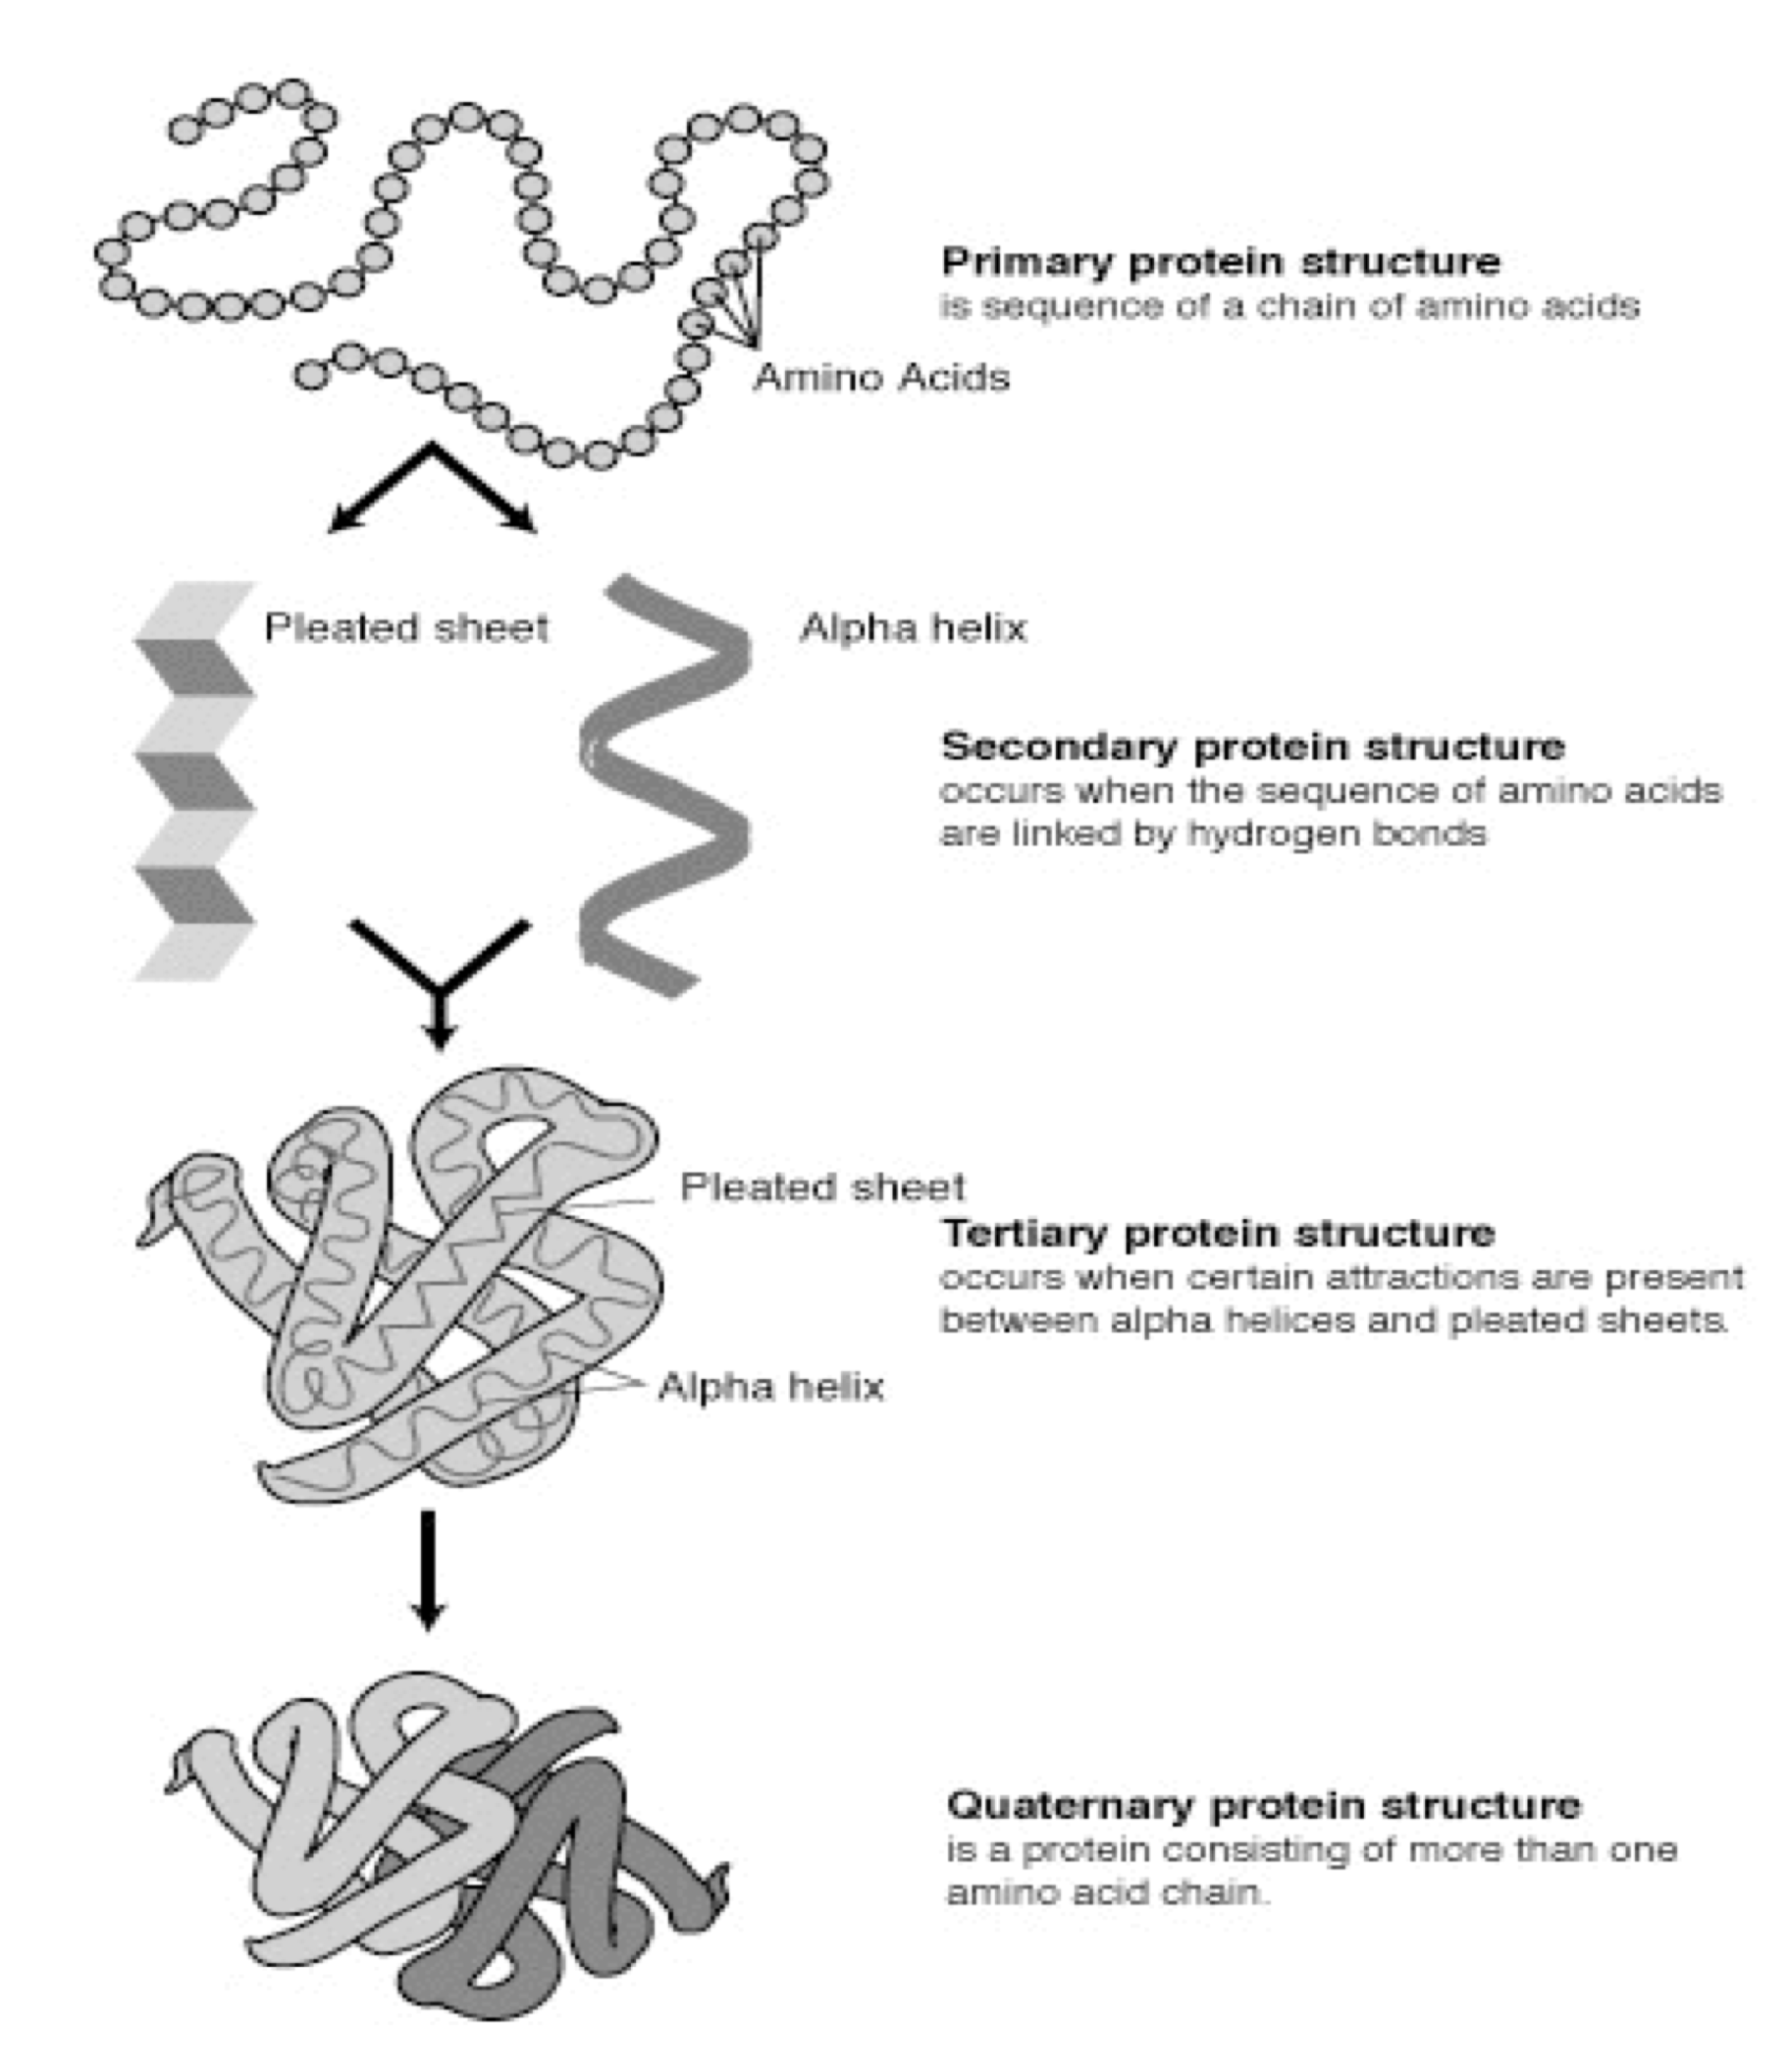
\includegraphics[width=0.5\textwidth]{Proteine.png}
\end{center}
\paragraph{La struttura 3D di una proteina è molto complessa} La determinazione della
struttura 3D di proteine è un settore di ricerca molto attivo,
come mostra la crescita esponenziale di strutture depositate nel Protein Data Bank.\\
\section{Il cosmo "omico"}
\subsection{La genomica} 
\begin{itemize}
    \item \underline{Genoma:} Insieme dei geni di un organismo.
    \item \underline{Genomica:} scienza che se ne
    occupa.
    \item \underline{Genoma Umano:} Sequenziato
    completamente nel 2003.
    \item \underline{Occorre localizzare:} Elementi
    Funzionali:
    \subitem{-} Regioni 'utili' → geni;
    \subitem{-} Sequenze codificanti,
    comprendere i meccanismi che
    regolano l'espressione, scoprire
    la funzione, e cercare
    d'intervenire specificamente su
    quest'ultima.
\end{itemize}
Il costo del sequenziamento del genoma oggi è alla portata di ciascun individuo.
\subsection{Trascrittomica}
\begin{itemize}
    \item \underline{Trascrittoma:} l'insieme di tutti i
    trascritti (RNA messaggeri,
    mRNA)
    \item \underline{Trascrittomica:} scienza che se ne
    occupa.
    \item \underline{Occorre localizzare:} Profili di
    espressione:
    \subitem{-} più dinamico del genoma
    \subitem{-} microarrays monitorano i
    livelli di espressione di migliaia
    di geni allo stesso tempo.
    Mirano ad individuare
    correlazioni e legami tra
    espressione genica, attivazione
    e inibizione.
    Esempi: studio nella
    differenziazione di cellule
    staminali o evoluzione di
    tumori.
\end{itemize}
\subsection{Proteomica}
\begin{itemize}
    \item \underline{Proteoma:} l'insieme di tutte le
    proteine in un sistema biologico o
    nel suo genoma
    \item \underline{Proteomica:} scienza che se ne
    occupa.
    \item \underline{Occorre localizzare:} sia le
    proteine codificate dai geni che le
    possibili modificazioni post-
    traduzionali (gruppi prostetici,
    multidomini, fosforilazione, ecc).
    \item Alcune tecniche
    \subitem{-} Gel:
        \subsubitem 1° dimensione punto
        isoelettrico
        \subsubitem 2° massa molecolare
    \subitem{-} Spettrometria di massa:
    identifica una proteina in base
    al suo rapporto massa/carica in
    seguito a ionizzazione
\end{itemize}
\subsection{Genomica Strutturale}
\begin{itemize}
    \item \underline{Genomica strutturale:}
    determinazione della struttura
    terziaria e quaternaria (3D e
    domini) delle proteine.
    \item \underline{Tecniche:} cristallografia, NMR,
    homology modeling, cryoEM
    (microscopia crioelettronica)
    + AlphaFold (basato su AI)
    \item La struttura terziaria di una
    proteina è essenziale per
    determinarne la funzione
\end{itemize}
\subsection{Farmaco-genomica}
\begin{itemize}
    \item \underline{Farmacogenomica}: mira a
    prevedere la reazione di ciascun
    individuo verso un principio attivo
    in base al suo genotipo.
    \item \underline{Obiettivo:} creare terapie
    farmacologiche personalizzate
    per ottimizzare il risultato
    minimizzando gli effetti
    collaterali.
    \item Esempio: previsione di gravi
    reazione avverse a Abacavir
    nella terapia dell'HIV
\end{itemize}
\section{L'evoluzione ed il confronto tra sequenze}
Un allele (variante di un gene presente contemporaneamente
nella popolazione) può essere generato, fissato o mutare nel
tempo.\\
\textbf{Uno degli obiettivi in senso lato della bioinformatica è
stabilire se l'analisi dell'informazione riguardo a due
oggetti biologici (e.g. geni o proteine) permette di stabilire
una relazione di OMOLOGIA, cioè di discendenza da un
antenato comune}
Due sequenze che vengono separate fisicamente (per speciazione,
duplicazione ecc.) non si scambiano piu' "informazione" ed evolvono
indipendentemente, accumulando mutazioni. Spetta a noi trovare i tratti
conservati dal comune antenato.\\
Un modo per muoversi in tal direzione è allineare le sequenze e determinare la
percentuale di identita' o sequence identity (s.i.) (rapporto, in \% tra il numero
dei amminoacidi/basi identici rispetto al totale) o comunque il grado di similitudine.
Di norma, sequenze nucleotidiche non correlate hanno una s.i. ~50\%; sequenze
amminoacidiche non correlate hanno una s.i. ~20\%. Se tali valori aumentano,
aumenta la probabilità che le sequenze siano omologhe. Ma tale indice dovrebbe
tener conto anche della lunghezza delle sequenze.
Una s.i. del 90\% fra due sequenze di 100 a.a. ha un significato diverso rispetto alla
stessa s.i. su sequenze di 30 a.a.
\textbf{Allineare due sequenze significa stabilire se tra esse sussiste una
relazione di omologia}
\begin{titlepage}
    \begin{center}
        \vspace*{1cm}
        \LARGE
        \textbf{Lezione 2: Basi di Dati Biologiche}
        
    \end{center}
\end{titlepage}
\section{Le Basi di Dati Biologiche}
Il concetto di informazione è strettamente connesso a quello di dato e di
struttura.
Il dato è un osservabile (insieme di numeri, caratteri, simboli…)
La struttura è l' organizzazione ordinata di dati che ne consente
l'apprendimento.\\
Una banca dati è l'insieme di dati elementari, omogenei,
ordinati e fruibili. In altre parole: è una collezione
organizzata di dati
Esempio: elenco telefonico. L'informazione è strutturata in campi (nome,
cognome ecc.). Ogni persona con i propri dati è un record.
I dati biologici necessitano di un'organizzazione. Primo tentativo:
Margaret Dayhoff (1925-1983): raccolse, nel 1965, le sequenze di
65 proteine (lavoro pioneristico per il tempo!)
Le tecniche di sequenziamento rapido ed i progetti \textit{-omici} hanno
prodotto una quantita' esplosiva di dati, anche di sequenze
L'avvento di Internet ha facilitato di gran lunga l'acquisizione e la
distribuzione dell'informazione biologica in banche dati.\\
\subsection{Introduzione}
\begin{itemize}
    \item Sono collezioni di dati:
        \subitem{-} strutturati
        \subitem{-} indicizzati
        \subitem{-} aggiornati
        \subitem{-} interconnessi
    \item I database biologici sono legati a strumenti per:
        \subitem{-} recuperare records al loro interno 
        \subitem{-} aggiornare il database
        \subitem{-} combinare le informazioni
    \item Ci sono 6 principali categorie di basi di dati biologiche:
        \subitem{-} basi di dati di sequenze
            \subsubitem DNA
            \subsubitem RNA
            \subsubitem Proteine
        \subitem{-} basi di dati per il mapping
            \subsubitem geni
            \subsubitem cromosomi
            \subsubitem \dots
        \subitem{-} Strutture3d (PDB)
        \subitem{-} Trascrittomica
        \subitem{-} Funzionali (KEGG)
        \subitem{-} Per la letteratura (PubMed), ontologies (GO), \dots
\end{itemize}
A gennaio di ogni anno il Nucleic Accids Research pubblica un Database Issue, a gennaio:
\begin{itemize}
    \item nel 2020 contiene 89 nuovi database e l'aggiornamento di 90 database
    \item classificati nelle seguenti categorie
        \subitem{-} Nucleotide Sequence Databases
        \subitem{-} RNA sequence databases
        \subitem{-} Protein sequence databases
        \subitem{-} Structure Databases
        \subitem{-} Genomics Databases (non-vertebrate)
        \subitem{-} Metabolic and Signaling Pathways
        \subitem{-} Human and other Vertebrate Genomes
        \subitem{-} Human Genes and Diseases
        \subitem{-} Microarray Data and other Gene Expression Databases
        \subitem{-} Proteomics Resources
        \subitem{-} Other Molecular Biology Databases
        \subitem{-} Organelle databases
        \subitem{-} Plant databases
        \subitem{-} Immunological databases
        \subitem{-} Cell biology
        \subitem{-} COVID-19 databases
\end{itemize}
Le banche dati si strutturano e si integrano per favorire lo studio del dogma centrale della biologia.
Tre enti al mondo sono i principali.
\begin{itemize}
    \item EMBL
    \item NCBI
    \item DDBJ
\end{itemize}
Integrando collegamenti esterni (Swiss-prot, ExPASy,
UCSC, ecc, ecc…) sono un punto ideale di partenza.
\subsection{Dati di Sequenza}
Che dati si possono trovare?
\begin{itemize}
    \item Principalmente sono presenti
        \subitem{-} sequenze di caratteri (nucleotidi, amminoacidi)
        \subitem{-} o strutture
    \item L'uso della rappresentazione dei dati biologici di
    varia natura come sequenze è la forma di gran lunga
    più diffusa.
    \item Sequenze di DNA: formate da 4 tipi di lettere (a,c,g,t), convenzionalmente minuscole
    \item Sequenze di RNA: formate da 4 tipi di lettere (A,C,G,U), convenzionalmente maiuscole
    \item Sequenze proteiche: formate da 20 lettere (A, C, D, E, F, G, H, I,K, L, M, N, P, Q, R, S, T, V, W, Y), convenzionalmente maiuscole
\end{itemize}
Il formato FASTA-Pearrson: 
\begin{itemize}
    \item Rappresentazione mediante testo di sequenze nucleotidiche o
    peptidiche (lettere MAIUSCOLE).
    \item La prima riga (di lunghezza arbitraria) è preceduta da ">" e rappresenta
    la descrizione della sequenza.
    \item Le linee precedute da ">" o ";" sono considerate di commento e non
    vengono interpretate come dato di sequenza
    \item Le linee successive (ciascuna di 80 caratteri) rappresentano la
    sequenza.
    \item Un file fasta può avere estensione (non c'è uno standard)
\end{itemize}
Il formato XML (eXtensible Markup Language).
\begin{itemize}
    \item Replica la struttura logica del record nella banca dati
    \item I tag permettono di delimitare e definire campi e sottocampi
\end{itemize}

\section{NCBI}
NCBI (National Center for Biotechnology Information) presso il National Institute of Health. Offre accesso a tante risorse di vario tipo:
\begin{itemize}
    \item Sequenze geniche e proteiche
    \item Strutture terziarie
    \item Genomi completi
    \item Pathways
    \item EST (expressed sequence tags)
    \item Profili trascrittomici
    \item Cataloghi tassonomici
\end{itemize}
Fornisce accesso a numerosi database attraverso il sistema Entrez:
\begin{itemize}
    \item GenBank
    \item Swissprot
    \item PubMed
    \item GEO 
    \item \dots
\end{itemize}
Fornisce accesso anche a diversi software bioinformatici.
\subsection{Com'è strutturato il database}
Una ricerca qualunque dall'home page apre ENTREZ,
interfaccia per l'accesso ai database presenti in NCBI.\\
\begin{itemize}
    \item PubMed è l'interfaccia di accesso a
    MEDLINE.
    Con I suoi
    \subitem{-} 20 milioni di record fino agli anni '50
    \subitem{-} 4600 riviste da più di 70 paesi\\
    È la banca dati per la letteratura
    biomedica più completa.
    (Accessibile anche tramite EBI tramite 17 CiteXplore)
    \item Nucleotide è un database che
    raccoglie sequenze da diversi altri
    database di NCBI.
    Per sequenze nucleotidiche
    \subitem{-} EST ( expressed sequence tag )
    \subitem{-} GSS ( genome sequence surveys
    Gene è orientato ai geni, ai loci
    altre sequenze, B act A rtif C hromosome ,
    Y east A rtif C hromosome ,\dots)\\
    Inoltre:
    \subitem{-} RefSeq ( sistema di
    identificazione )
    \subitem{-} Unigene ( sequenze raggruppate )
    \subitem{-} UniProt ( proteine )
    \item Gene è orientato ai geni, ai loci
    \item Proteins è la sezione focalizzata sulle
    proteine, alle quali possono
    corrispondere strutture
    \item PubChem dedicato ai composti chimici
    \item In Genome genomi completi con riferimenti alla
    ricerca effettuata, varianti genomiche,
    ecc
    \item Informazioni su profili di espressione
    genica in diverse condizioni, modifiche
    post-traduzionali
    GEO (Gene Expression Omnibus)
    repository
\end{itemize}
GenBank è la banca dati di tutte le sequenze in NCBI (sincronizzata con
EMBL e DDBJ). Le sequenze derivano da diverse fonti e tipi:
\begin{itemize}
    \item Geni (regioni di regolazione, esoni, introni: unità ereditarie)
    \item EST (Expressed Sequence Tags)
    brevi segmenti di DNA trascritti e sequenz. da cDNA (ottenuto da
    mRNA retrotrascritto)
    \item STS (sequence tagged site, dove l'informazione genetica è mappata
    fisicamente)
    \item GSS (Genome Survey Sequence, vettori sequenze solo parzialmente sequenziate)
    \item HTGS (High Throughput Genomic Sequence, sequenze prodotte da tecniche di
    seconda generazione per il sequenziamento veloce, messe qui in “preview”)
    \item Sequenze di proteine (sezione nr, non redundant)
\end{itemize}
Così tanto materiale ha provocato l'esigenza di ordine: \textbf{RefSeq}.\\
RefSeq è stato ideato per far corrispondere a ciascun trascritto
normalmente prodotto da un gene e a ciascuna proteina una sequenza di
riferimento, un identificatore (accession number).\\
Altri esempi di identificatori NON RefSeq sono:
\begin{itemize}
    \item X02775 GenBank/EMBL/DDBJ nucleotidic sequence
    \item Rs7079946 dbSNP (single nucleotide polymorphism)
    \item N91759.1 An expressed sequence tag
    \item AAC02945 GenBank protein
    \item Q28369 SwissProt protein
    \item 1KT7 Protein Data Bank structure record
\end{itemize}
Refseq fornisce un identificatore per la sequenza di riferimento, curato dal
personale dell'NCBI.\\
formati principali degli id RefSeq sono:
\begin{itemize}
    \item Complete genome/chromosome/plasmid N\textbf{C}$\_\#\#\#\#\#\#$
    \item Genomic contig (segmenti sovrapposti di DNA segments che rappresentano una sequenza consenso) N\textbf{T}$\_\#\#\#\#\#\#$
    \item mRNA (DNA format) N\textbf{M}$\_\#\#\#\#\#\#$
    \item Protein N\textbf{P}$\_\#\#\#\#\#\#$
\end{itemize}
\paragraph{Un primo esempio di ricerca - L'Emoglobina}
Una delle prime proteine ad essere studiata (anni '30 e '40, da Mulder, Liebing et al.).\\
È stata la prima proteina ad essere usata negli allineamenti multipli di sequenza:
voglio fare dei confronti di sequenze (ad esempio per confrontare la stessa proteina prodotta da diverse specie). Con le prime tecniche di sequenziamento abbiamo scoperto che è stata localizzata in due loci, uno sul cromosoma 16 (subunità alfa) e 11 (subunità beta). I due geni sono regolati sia in base all'età che in base ai diversi tessuti.\\
È quindi un problema complesso che ha poi originato una serie di considerazioni.
La mioglobina, una globina (struttura globulare a 8 eliche)
che lega l'ossigeno nei tessuti muscolari, è stata la prima
proteina la cui struttura tridimensionale è stata risolta
tramite cristallografia.\\
L'emoglobina è un tetramero (due catene alfa e due beta negli
adulti) è il principale trasportatore di ossigeno nei vertebrati.
Assieme alla mioglobina è stata usata nei primi studi sugli
allineamenti multipli.\\
Negli anni '80 con le prime tecniche di sequenziamento è stata
localizzata in due loci, uno sul cromosoma 16 (subunità alfa) e 11
(subunità beta). I due geni sono regolati sia in base all'età che in
base ai diversi tessuti.
\subsubsection*{Ricerca dell'emoglobina}
\begin{enumerate}
    \item Inseriamo "beta globin" nella barra di ricerca
    \item Seguiamo poi il link a "Gene"
    \item Entrez Gene (ex LocusLink) è un portale curato che descrive loci genetici
        \subitem{-} nomenclatura
        \subitem{-} alias
        \subitem{-} accession numbers
        \subitem{-} fenotipi
        \subitem{-} OMIM (ereditarietà dei caratteri)
        \subitem{-} HomoloGene
        \subitem{-} mappatura sul genoma
        \subitem{-} collegamenti esterni
    \item In generale ad oggi quesa ricerca trova 126 entries
    \item Intestazione: Entrez Gene, Noa: "Official Symbol", HBB per la beta globina
    \item Limitiamoci alla ricerca per Homo Sapiens (selezionando sulla destra da Results by taxon)
    \item Cliccando la specie si aggiorna automaticmente la stringa di ricerca: {\ttfamily(beta globin) AND "Homo sapiens" [ porgn:\_txid9606 ]}
    \item Con il limite Homo Sapiend le entries sono solo 41
    \item Apriamo la prima entry
    \item Sulla dx in basso troviamo numerosi link a database esterni
    \item Abbiamo una sezione sulle regioni genomiche, una sulla bibliografia
    \item Sezione interessante: GeneRif (intended to facilitate access to publications documenting experiments that add to our understanding of a gene and its function)
    \item E ancora Fenotipi, Variazione Genica, Pathways per Biosistemi e Interazioni note con altri geni.
    \item Ontologia: (fondamentale per sistemi automatici di apprendimento). Classificazione
    e organizzazione dei dati in categorie predefinite così da agevolare l'individuazione di
    analogie e caratteristiche primarie. Può essere di diversi tipi, ma la principale distingue:
        \subitem{-} Funzione molecolare
        \subitem{-} Localizzazione cellulare
        \subitem{-} Processo biologico
    \item Catalogazione RefSeq (a fine pagina)
\end{enumerate}
\subsection{Operatori Booleani}
\subsubsection{Operatore AND (\&)}
Restringe il campo di ricerca, inserendo ad es. la stringa:
{\ttfamily equus caballus AND hemoglobin alpha}\\
La banca dati ci mostrerà una lista di sequenze proteiche i cui campi di
descrizione contengono entrambe le parole. Quindi le sequenze proteiche
del cavallo che non contengono nella descrizione la parola hemoglobin
non vengono selezionate.
\subsubsection{Operatore OR (|)}
Estende il campo di ricerca, digitando ad esempio:
Restringe il campo di ricerca, inserendo:
{\ttfamily homo sapiens OR mus musculus}\\
Otterremo una lista di sequenze i cui campi contengono la parola homo
sapiens o la parola mus musculus.
L'operatore allarga l'insieme
delle sequenze che incontrano le nostre esigenze.
\subsubsection{Operatore NOT (!)}
Restringe il campo di ricerca, inserendo:
{\ttfamily homo sapiens NOT hemoglobin}
Richiederemo sequenze i cui campi contengono la parola homo sapiens
ma non la parola hemoglobin.
\subsubsection{Combinazione di Operatori Booleani}
Gli operatori booleani si possono combinare, vengono letti da sinistra a
destra. Per questo sono utili le parentesi. Ad esempio: globin AND promoter OR enhancer produce quasi 5000
hits. Ma se si scrive globin AND (promoter OR enhancer) se ne
ottengono circa 70.\\
Altre possibilità sono:
\begin{itemize}
    \item Specificare un organismo (human, nella query:
    human[ORGN]
    \item Usare l’asterisco: glob * restituisce tutte le entry che
    contengono una stringa che inizia per “glob”
    \item Usare le virgolette “” . La ricerca di “toxin B1” restituirà le
    entries che contengono esattamente la stringa intera.
    \item \dots
\end{itemize}
\subsection{Nel dettaglio}
\paragraph{Homologene}
la risorsa ideale per individuare gruppi
di geni omologhi negli eucarioti presenti in NCBI
\paragraph{OMIM}
Catalogo di geni umani e disordini genetici
\paragraph{SNP}
Single Nucleotide Polimorfism
\newpage
\section{Proteine - Le banche dati proteiche più usate}
\paragraph{Uniprot}
(Universal Protein Resource) raccoglie le informazioni dei database:
\begin{enumerate}
    \item Swiss-prot (SIB)
    \item TrEMBL (EBI) 
    \item PIR
\end{enumerate} 
Offre la possibilità di effettuare Text
Search o Blast Search. Viene curato anche un database NON RIDONDANTE
(UniRef).
\paragraph{Swissprot}
Molto curato e detagliato, con annotazioni circa funzione, struttura, modificazione e altre informazioni utili.
\paragraph{TrEMBL}
È la traduzione in silico di ogni entry codificante del database primario dell'EMBL, non è accurato, ma è ricchissimo.
\paragraph{PIR}
È il discendente diretto del database della Dayhoff, è curato a mano e le annotazioni sono molto ricche e precise.
\subsection{NCBI Protein - non molto ricco}
Entrez Protein: Contiene diverse informazioni su proteine
\begin{itemize}
    \item 147 amminoacidi
    \item PRI: primates
    \item $NP\_000509$ (protein accession number)
    \item $NM\_000518.4$ (mRNA, RefSeq)
    \item Riferimenti bibliografici
    \item Sequenze FASTA (Opzione Display)
    \item Siti di modificazione post-traduzionale (AA94, AA121)
    \item Riferimenti ad altri database
    \item Sequenza amminoacidica (1 lettera)
\end{itemize}
È un record non molto ricco dal punto di vista dei dati delle proteine.
\subsection{Uniprot}
Uniprot è il più completo database centralizzato per le sequenze proteiche.\\
È organizzato su 3 livelli:
\begin{enumerate}
    \item Uniprot Knowledge Base
        \subitem{-} Swiss-Prot (curato)
        \subitem{-} TrEMBL (automatico)
    \item UniProt Reference
    clusters (UniRef)
        \subitem{-} Cluster di proteine che
        condividono il 50\%, 90\%,
        100\% di identità di
        sequenza
    \item UniProt Archive (UniParc)
        \subitem{-} Archivio di sequenze
        proteiche stabile, non
        ridondante, da diverse 58 fonti
\end{enumerate}
\subsubsection{Struttura del database}
Nella homepage abbiamo la classica barra di ricerca e subito sotto i link di accesso alle diverse informazioni contenute in Uniprot.\\
\paragraph{Un esempio di ricerca}
\begin{enumerate}
    \item Inseriamo "{\ttfamily hbb}" nella barra di ricerca.
    \item Sulla sinistra possiamo selezionare gli organismi a cui restringere la ricerca. Selezioniamo Humans.
    \item Questo aggiornerà automaticamente la stringa di ricerca: {\ttfamily hbb AND organism: "Homo sapiens (Human) [9605]"}
    \item Selezioniamo la prima entry.
    \item Sulla sinistra troviamo la tavola con tutti i contenuti disponibili.
    \item Tra i più importanti abbiamo: "Function" (che specifica la funzione della proteina), "Pathology \& Biotech", "Expression", "Interaction", "Family \& Domains", \dots
    \item In "Structure" e altre sezioni troviamo i link a PDB (Protein Data Bank), database di strutture proteiche.
    \item In "Sequence" troviamo tutta la sequenza proteica, scaricabile in formato FASTA.
    \item Abbiamo inoltre vari link di collegamento ad altri database di sequenze (EMBL,GeneBank, DDBJ), varianti, \dots
\end{enumerate}
\subsection{ExPASy}
(Expert Protein Analysis System)\\
È una risorsa curata, espressione del SIB (Swiss Institute of
Bioinformatics). Principalmente dedicata alle proteine.\\
La risorsa principale che ha prodotto è SwissProt (confluita in Uniprot). Rimane un punto di riferimento per molti tools. 

\begin{titlepage}
    \begin{center}
        \vspace*{1cm}
        \LARGE
        \textbf{Lezione 3: Allineamenti di Sequenze - concetti e algoritmi}

    \end{center}
\end{titlepage}


\begin{titlepage}
    \begin{center}
        \vspace*{1cm}
        \LARGE
        \textbf{Lezione 6: Allineamenti Multipli di Sequenze}

    \end{center}
\end{titlepage}
\section{Allineamento multiplo di sequenze}
\subsection{Visione Generale}
\subsubsection{Una definizione}
Un allineamento multiplo è una collezione di tre o più sequenze proteiche (o nucleotidiche) parzialmente o completamente allineate
\begin{itemize}
    \item I residui e le zone omologhe sono allineate in colonne per tutta la lunghezza delle sequenze
    \item Il senso dell'omologia dei residui è evoluzionistico
    \item Il senso dell'omologia dei residui è strutturale
\end{itemize}
Si tratta di un argomento di ricerca attivo dagli anni '90.
\subsubsection{Alcuni fatti}
Non c'è necessariamente un allineamento "corretto" per una famiglia di proteine.\\
\textbf{Perchè?}
    \begin{itemize}
        \item Le sequenze di proteine evolvono
        \item Le corrispondenti strutture tridimensionali evolvono, anche se più lentamente
        \item Può essere particolarmente difficile identificare i residui che si sovrappongono nello spazio (strutturalmente) in un allineamento multiplo di sequenze.
    \end{itemize}
\hl{Due proteine che condividono il 30\% di identità di sequenza avranno circa il 50\% dei residui sovrapponibili nelle due strutture}
\subsubsection{Caratteristiche utili per realizzzarlo}
Alcuni residui allineati, come cisteine che formano ponti disolfuro, o i triptofani, possono essere altamente conservati
    \begin{itemize}
        \item Ci possono essere motivi conservati come un dominio transmembrana
        \item Alcune caratteristiche come le strutture secondarie, siti attivi e di legame per ligandi o complessi sono spesso conservate
        \item Ci possono essere regioni con inserimenti o delezioni propagati in parte della famiglia.
        \item I principi che vedremo sono focalizzati sulle proteine ma sono validi in generale anche per sequenze nucleotidiche.
    \end{itemize}
\subsubsection{Utilizzi e Vantaggi}
    \begin{itemize}
        \item Il MSA è più sensibile di quello a coppie nel rilevamento di omologie, per questo è uno strumento essenziale nella costruzione di modelli strutturali per omologia
        \item L'output di BLAST può assumere la forma di un MSA, e possono essere individuati residui conservati o motivi
        \item In un MSA si possono analizzare i dati di una popolazione
        \item Una singola query può essere cercata contro un database di MSA (ad esempio Pfam)
        \item Le regioni regolatorie dei geni sono spesso identificabili da MSA
    \end{itemize}
\subsection{Metodi}
I metodi esatti non vengono trattati in questa sede: non ci sono soluzioni efficienti e già con 5 sequenze il tempo di computazione è eccessivo (esponenziale)
\subsubsection{Metodi Euristici}
\hl{\textbf{Metodi progressivi}}: usano un albero guida (analogo ad un albero filogenetico) per determinare come combinare uno per uno allineamenti a coppie
(progressivamente) per creare un allineamento multiplo.\\
\small{Esempi: CLUSTAL OMEGA (W), MUSCLE (usato da HomoloGene)}
\paragraph{Il MSA progressivo di Feng-Doolittle (1987) alla base di Clustal (W) avviene in 3 fasi}
\begin{enumerate}
    \item Realizzare una serie di allineamenti a coppie globali (Needleman e Wunsch, algoritmo di programmazione dinamica) di cui si calcola la distanza (matrice delle distanze)
    \item Creare un albero guida a partire dalla matrice delle distanze
    \item Allineare progressivamente le sequenze
\end{enumerate}
\textbf{MSA progressivo, fase 1 di 3:}\\
\normalsize{generare allineamenti a coppie globali}\\
\small{Esempio: allineare 5 globine (1, 2, 3, 4, 5).}\\
\paragraph{\hl{Primo step:} a due a due e valutare gli score di ogni possibile allineamento a coppie\\}
\textbf{Numero di allineamenti a coppie necessari per coprire tutte le possibili combinazioni}
\begin{itemize}
    \item Per n sequenze, (n-1) (n) / 2
    \item Per 5 sequenze, (4) (5) / 2 = 10
    \item Per 200 sequenze, (199) (200) / 2 = 19.900
\end{itemize}…Quindi per molte sequenze ClustalW è molto lento ed è preferibile usare metodi più veloci (MUSCLE è molto veloce).
\paragraph{\hl{Secondo step:} albero guida\\}
\textbf{Convertire i punteggi di similitudine in punteggi di distanza:} è matematicamente più semplice, oltre che più intuitivo, lavorare con le distanze. Una semplice definizione di distanza è data dalla percentuale di
residui diversi (100- SI in \%) che viene inserita nella matrice delle distanze.
\begin{itemize}
    \item Dalla matrice delle distanze si calcola l'albero guida con il metodo di clustering neighbor joining che vedrete nel modulo 2.
    \item Vediamo un semplice esempio di clustering e costruzione di albero guida
\end{itemize}
\paragraph{Il clustering alla base di CLUSTAL(W)} È una matrice di distanze, minore è il numero, maggiore è la similitudine.
\textit{Nota: tutte le distanze tra la I e la IV riga sono minori di quelle riportate nella V}
%inserire foto 
\begin{itemize}
    \item Tutte le sequenze vengono poi allineate progressivamente, seguendo le indicazioni dell'albero
    guida: prima si allineano le più simili (vicine) e poi progressivamente le più distanti.
    \item A ogni passaggio si utilizza un algoritmo dinamico di allineamento molto efficiente che accoppia sequenze o gruppi di sequenze
    \item Il MA è composto a partire a tanti allineamenti a coppie, anche fra gruppi di sequenze.
    \item{} \textit{Nota: Le indel presenti negli allineamenti già effettuati restano fisse.}
    \item Come allineare pogressivamente due gruppi di sequenze? Si usa sempre una matrice. È simile all'allineamento dinamico di due sequenze visto.
    \item Lo score S in ogni
    casella è la media degli score ottenuti confrontando tutte le possibili coppie di a.a. nella riga e colonna
    corrispondenti (secondo ad es. BLOSUM62)
    \item 
\end{itemize}


\begin{titlepage}
    \begin{center}
        \vspace*{1cm}
        \LARGE
        \textbf{Domande stile esame}

    \end{center}
\end{titlepage}

\section{Domande sull'introduzione}
\Large
\begin{enumerate}
    \item Differenza tra omologia e similitudine. È possibile che due proteine abbiano unìidentità di sequenza del 57\% e una similitudine del 21\%? Perchè?
\end{enumerate}

\section{Domande sulle banche dati}
\begin{enumerate}
    \item ) Cos’è Uniprot? Oltre ad una descrizione generale si descrivano i suoi livelli e si elenchino almeno 5 sezioni che si possono trovare nelle pagine delle singole proteine (entry). Si descrivano inoltre brevemente i database PDB e ExPASy. Cosa hanno in comune queste tre risorse?
    \item Si citino e discutano brevemente 4 banche dati presenti in NCBI. Se possibile escludere NCBI protein.
    \item Si descrivano le banche dati NCBI Gene, Unigene e Genbank. Inoltre, in che relazione sono tra di esse?
    \item  Descrivere Uniprot, Pfam, Prosite, CATH e PDB, con particolare attenzione alla più importante tra di esse (qual è?)
    \item Cos’è Pubmed? Descrivere la banca dati, i suoi contenuti, e gli strumenti messi a disposizione degli utenti (illustrati a lezione), sia per la ricerca che per la gestione dei risultati.
    \item Descrivere brevemente le caratteristiche del Protein Data Bank ed il contenuto di un file pdb.
    \item Si descrivano il formato FASTA, il formato ASN.1 e il formato XML nell'ambito della bioinformatica.
    \item 
\end{enumerate}


\end{document}